%----------------------------------------------------------------------------
\chapter{Background} \label{background}
%----------------------------------------------------------------------------


%----------------------------------------------------------------------------
\section{Cloud Computing}
%----------------------------------------------------------------------------

\begin{itemize}
	\item \cite{AboveTheClouds}
	\begin{itemize}
		\item refers to both the applications delivered as services over the Internet and the hardware and systems software in the data centers that provide those services (these are often referred as software as a service) - here we focus on the applications
		\item cloud = data center hardware and software
		\item public cloud vs private cloud
		\item cloud pros - appearance of infinite computing resources, elasticity (to serve varying demand, or when demand is unknown), pay per use, transference of risk (of operation and of over/underprovisioning)
		\item 
	\end{itemize}
\end{itemize}

%----------------------------------------------------------------------------
\subsection{Software as a Service}
%----------------------------------------------------------------------------

\begin{itemize}
	\item https://en.wikipedia.org/wiki/Software\_as\_a\_service
	\begin{itemize}
		\item software delivery model (wikipedia)
		\item software is licensed on a subscription basis (wikipedia)
		\item software is centrally hosted (wikipedia)
	\end{itemize}
	\item \cite{AboveTheClouds}
	\begin{itemize}
		\item simplified software installation, maintainence, centralized control over versioning
		\item users can access the service anywhere, anytime, share and collaborate easily, keep data stored safely
		\item cloud computing allows deploying, scaling SaaS on demand
	\end{itemize}
	\item \cite{SaaSOppRisk}
	\begin{itemize}
		\item The SaaS model evolved from the application service provisioning (ASP) model, which emerged in the late 1990s as an on-demand software delivery option for (on-premise) commercial off-the-shelf application development. The ASP model involved vendor hosting, as well as managing and delivering application capabilities remotely from a data center accessed via the Internet. Technical issues that held ASP back during the 1990s included the initial design problems (i.e., few software applications were designed to be remotely accessible at that time), limited bandwidth availability, and slow Internet speeds. 
		\item multitenant architecture, there is only a single instance of the common code and data definitions of a given application on the vendor's server.
		\item the applications and infrastructure are shared across customers in the SaaS model
		\item SaaS model constrains clients' customization options of the software's main functionality and data structures
		\item it provides the vendor with more control over future development: 
	\end{itemize}
	
\end{itemize}


%----------------------------------------------------------------------------
\section{Microservices}
%----------------------------------------------------------------------------

before this, monolithic applications were popular

\begin{itemize}
	\item one deployment unit with many responsibilities
	\item tight coupling of different use-cases
	\item scalability issues
	\item vendor and technology lock in for the entire business application
\end{itemize}

----

\begin{itemize}
	\item \cite{MicroservicesMF}
	\begin{itemize}
		\item in short, the microservice architectural style is an approach to developing a single application as a suite of small services, each running in its own process and communicating with lightweight mechanisms, often an HTTP resource API. These services are built around business capabilities and independently deployable by fully automated deployment machinery. There is a bare minimum of centralized management of these services, which may be written in different programming languages and use different data storage technologies.
		
		Characteristics of a Microservice Architecture
		
		\item Componentization via Services
		\begin{itemize}
			\item here, a component is a unit of software that is independently replaceable and upgradeable.
			\item services are out-of-process (run in different processes, most likely on different machines - physical of virtual) components that communicate with mechanisms over the network
			\item services can be independently deployable (pros...)
			\item more explicit component interface
			\item Remote calls are more expensive than in-process calls, and thus remote APIs need to be coarser-grained, which is often more awkward to use (no free lunch)
		\end{itemize}
		\item Organized around Business Capabilities
		\item Smart endpoints and dumb pipes
		\begin{itemize}
			\item Applications built from microservices aim to be as decoupled and as cohesive as possible - they own their own domain logic and act more as filters in the classical Unix sense - receiving a request, applying logic as appropriate and producing a response.
			\item HTTP request-response, REST
			\item messaging over a lightweight message bus (RabbitMQ, Kafka)
		\end{itemize}
		\item Decentralized Governance
		\begin{itemize}
			\item no need to use the same technology stack for everything
			\item developers can use the right tools for each task and use-case
		\end{itemize}
		\item Decentralized Data Management
		\begin{itemize}
			\item each service maintains an own model of the world - its context is bounded so the component is only aware of the necessary information
			\item each component manages its own database, and databases can be accessed by other services only through their respective service - polyglot persistence
		\end{itemize}
	\end{itemize}
	\item \cite{ImplPatternsMicrosServices}
	\begin{itemize}
		\item Microservices is an application architectural style in which an application is composed of many discrete, network-connected components, termed microservices.
		\item the microservices approach stay focused on implementing clear business capabilities
		\item in the microservices architectural style, several smaller applications that each implement only part of the whole are built and packaged independently
		\item 5 simple rules drive the implementation of applications build using the microservices architecture
		\begin{itemize}
			\item Deploy applications as sets of small, independent services - one service per container
			\item Optimize services for a single function - this makes each service smaller and simpler to write and maintain (Rober Martin's "Single Responsibility Principle" \cite{RobertMartinOOP})
			\item Communicate via REST API and message brokers - limit options for simplicity, avoid tight coupling introduced by implicit communication through a database, ALL communication from service to service must be through the service API
			\item Apply Per-service CI/CD - it allows the different services to evolve at their own pace
			\item Apply Per-service HA/clustering decisions - The reality is that in a large system, not all services need to scale and can be deployed in a minimum number of servers to conserve resources. Others require scaling up to very large
			numbers.
		\end{itemize}
	\end{itemize}
	\item \cite{MicroservicesDocker}
	\begin{itemize}
		\item Microservices characteristics
		\begin{itemize}
			\item Small and focused - services should be modelled around specific business domain (not mimic organizational boundaries), each service should be treated as an independent application (own source code, CICD)
			\item Loosly coupled - Each microservice needs to be deployed as.needed without the necessary of coordination with other
			services’ owners
			\item Language-neutral - Microservices need to be built using technology that’s the developers are most comfortable with. The communication between the services is also language neutral, like HTTP or message brokers
			\item Bounded context - defines the details of a single domain (data model, domain model) and the integration points with other bounded contexts
		\end{itemize}
		\item Challenges in building a microservices architecture
		\begin{itemize}
			\item Failure Isolation - prefer quick failures, ability to determine where the failure happened
			\item Observability - health status, monitoring, logging - collect data and aggregate sensibly, helpful visualizations
			\item Automation requirement - as the number of services can grow rapidly
			\item High independence - 
			\item Testing - many moving parts, functional and non-functional aspects, distributed model
			\item Scaling - multiple instances, versions - many connections, service discovery mechanism, routing, configuration management issues
		\end{itemize}
	\end{itemize}
\end{itemize}


%----------------------------------------------------------------------------
\section{Dependability}
%----------------------------------------------------------------------------

Dependability of a computing system is the ability to provide service in which reliance can be justifiably placed \cite{DependabilityBMEMIT}. Meaning that based on conducting several analysis, evaluations and measurements it can be proofed that service satisfies the needs.

%----------------------------------------------------------------------------
\subsection{Attributes of Dependability} \label{dependability-attributes}
%----------------------------------------------------------------------------

Dependability is a complex extra-functional characteristic of a system that consists of multiple attributes (based on the lectures in Systems Engineering \cite{DependabilityBMEMIT} and the Fundamental Concepts of Dependability \cite{FundamentalConceptsOfDependability}):

\paragraph{Availability} - Availability describes the probability of correct service in a system. It also takes into account the time needed for repairs and maintenance tasks.

\paragraph{Reliability} - Reliability describes the probability of continuous correct service until the first failure. In case of mission critical systems, high reliability is an absolute requirement.

\paragraph{Safety} - A system is considered safe if it is free from unacceptable risk of harm. Harm can be defined in many different ways according to the domain in which the system operates.

\paragraph{Integrity} - Integrity assesses the absence of erroneous changes or alterations in the system. Integrity is a prerequisite for availability, reliability and safety as one cannot guarantee these attributes when there are misconfigurations in the system.

\paragraph{Maintainability} - Maintainability describes the possibility that the system is able to undergo repairs and improvements.


%----------------------------------------------------------------------------
\subsection{Dependability Metrics}
%----------------------------------------------------------------------------

The section above describing dependability presents well its compound nature, however, solely these definitions cannot be used to objectively assess the dependability of a given system in a deterministic way. Numerical representations of dependability -- so called dependability metrics -- are necessary in order to be able to conduct dependability analysis and measurements.

For sake of simplicity, one can use the notion that any given system has fundamentally two states, an Up and a Down state partitions. The Up partition stands for all the system states, where the system can provide correct service whereas the Down partitions denotes the states, where it cannot \cite{DependabilityBMEMIT}. It is important to mention, that providing correct service does not necessarily mean that the system is error free. Especially in case of highly distributed, dynamic environments, it is not feasible to guarantee the complete absence of errors for a long time. This leads to the fact that the essential question is not whether the system is error free, rather if it is able to function correctly and reliably.

The state of a system over time with respect to the before mentioned two state partitions can be visualized as shown in Figure \ref{fig:system_state_partitions}. The function \(s(t)\) shows the system partition at any given time. During the intervals labeled with \(u_i\) the system was in the Up partition while during the intervals labeled with \(d_i\) the system was in the Down partition.


\begin{figure}[h]
	\centering
	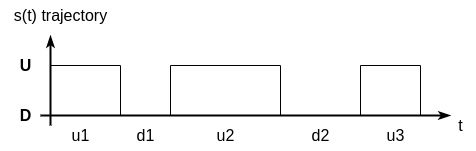
\includegraphics[width=100mm, keepaspectratio]{figures/system_state_partitions.png}
	\caption{ Partitioning the states of the system \cite{DependabilityBMEMIT} }
	\label{fig:system_state_partitions}
\end{figure}

%----------------------------------------------------------------------------
\subsubsection{Mean Values} \label{background-dep-metrics-mean-values}
%----------------------------------------------------------------------------

\paragraph{Mean Time to First Failure} - Mean Time to First Failure -- or MTFF -- denotes the expected time before a given system first encounters a failure that prevents providing correct service. MTFF is calculated with the following formula: \(E\{u_1\}\) and can be visualized using the previously mentioned state partitions as seen in Figure \ref{fig:mtff}.

\begin{figure}[h]
	\centering
	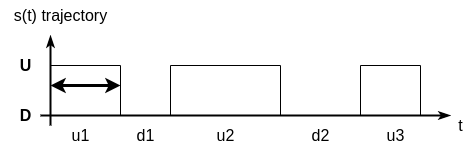
\includegraphics[width=100mm, keepaspectratio]{figures/MTFF.png}
	\caption{ Mean Time to First Failure \cite{DependabilityBMEMIT} }
	\label{fig:mtff}
\end{figure}

\paragraph{Mean Up Time} - Mean Up Time -- or MUT -- is the average duration of time periods during which the system is able to provide correct service. MUT is calculated with the following formula: \(E\{u_i\}\) and can be visualized using the previously mentioned state partitions as seen in Figure \ref{fig:mut}.

\begin{figure}[h]
	\centering
	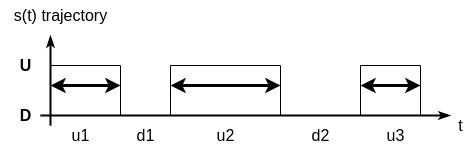
\includegraphics[width=100mm, keepaspectratio]{figures/MUT.png}
	\caption{ Mean Up Time \cite{DependabilityBMEMIT} }
	\label{fig:mut}
\end{figure}

\paragraph{Mean Down Time} - Mean Down Time -- or MDT -- is the average duration of time periods during which the system cannot provide correct service due to failures or maintenance. MDT is calculated with the following formula: \(E\{d_i\}\) and can be visualized using the previously mentioned state partitions as seen in Figure \ref{fig:mdt}.

\begin{figure}[h]
	\centering
	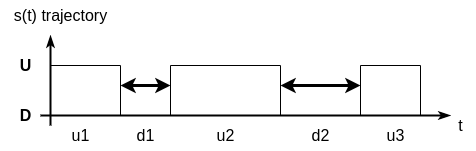
\includegraphics[width=100mm, keepaspectratio]{figures/MDT.png}
	\caption{ Mean Down Time \cite{DependabilityBMEMIT} }
	\label{fig:mdt}
\end{figure}

\paragraph{Mean Time Between Failures} - Mean Time Between Failures -- or MTBF -- denotes the average time between repairable failures of system \cite{KPIMetrics}. MTBF is calculated with the following formula: \(E\{u_i + d_i\} = E\{u_i\} + E\{d_i\}\) (the sum of MUT and MDT) and can be visualized using the previously mentioned state partitions as seen in Figure \ref{fig:mdt}.

\begin{figure}[h]
	\centering
	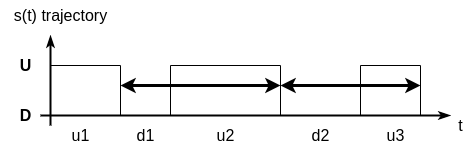
\includegraphics[width=100mm, keepaspectratio]{figures/MTBF.png}
	\caption{ Mean Time Between Failures \cite{DependabilityBMEMIT} }
	\label{fig:mtbf}
\end{figure}

%----------------------------------------------------------------------------
\subsubsection{Probability Functions} \label{background-dep-metrics-prob-funcs}
%----------------------------------------------------------------------------

\paragraph{Availability} - As mentioned earlier in Section \ref{dependability-attributes}, availability describes the probability of correct service in a system. Using the notion of Up and Down system partitions, availability can be calculated with the following formula:

\[
a(t) = P\{ s(t) \in U \}
\]

\paragraph{Reliability} - As mentioned earlier in Section \ref{dependability-attributes}, reliability describes the probability of continuous correct service until the first failure. Using the notion of Up and Down system partitions, availability can be calculated with the following formula:

\[
r(t) = P\{ s(t') \in U, \forall t' < t \}
\]


%----------------------------------------------------------------------------
\section{Kubernetes}
%----------------------------------------------------------------------------

Kubernetes is an open-source platform for managing containerized workloads and services, that facilitates both declarative configuration and automation \cite{KubernetesOverview}. Kubernetes orchestration allows IT professionals to build application services that span multiple containers, schedule those containers across a cluster, scale those containers, and manage the health of those containers over time \cite{KubernetesOverviewRH}.

Kubernetes brings a vast amount of useful features, but a thorough discussion concerning these is out of the scope of this work. However, a brief list is provided below for a clearer context \cite{KubernetesOverview}.

\paragraph{Service discovery and load balancing} - Kubernetes can expose a container using the DNS name or using their own IP address. If traffic to a container is high, Kubernetes is able to load balance and distribute the network traffic so that the deployment is stable \cite{KubernetesOverview}.

\paragraph{Automated rollouts and rollbacks} - Cluster administrators can describe the desired state for the deployed containers using Kubernetes, and it can change the actual state to the desired state at a controlled rate. For example, Kubernetes can automatically create new containers for a deployment, remove existing containers and adopt all their resources to the new container \cite{KubernetesOverview}.

\paragraph{Automatic bin packing} - Kubernetes can automatically schedule the containers of deployments to the nodes in the cluster and aims to achieve the best resource utilization over the whole cluster \cite{KubernetesOverview}.

\paragraph{Self-healing} Kubernetes can automatically restart containers that fail, replace containers, kill containers that do not respond to user-defined health check, and does not advertise them to clients until they are ready to serve \cite{KubernetesOverview}.

%----------------------------------------------------------------------------
\subsection{Cluster Architecture}
%----------------------------------------------------------------------------

\begin{figure}[h]
	\centering
	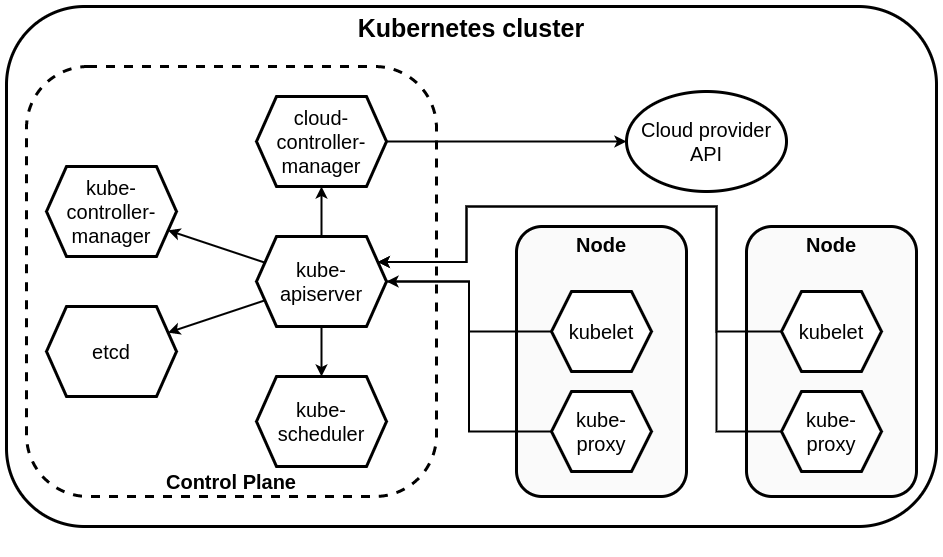
\includegraphics[width=130mm, keepaspectratio]{figures/kubernetes_components.png}
	\caption{Kubernetes Components \cite{KubernetesArchitecture}}
	\label{fig:kubernetes_components}
\end{figure}


A Kubernetes cluster consists of a set of worker machines, called nodes, and the control plane. The nodes can be physical or virtual machines depending on the environment and can run anywhere from private data centers to public cloud solutions and even on a single laptop. The control plane manages the worker nodes and the application workload on the cluster \cite{KubernetesArchitecture}. The overview of a Kubernetes cluster architecture can be seen in Figure \ref{fig:kubernetes_components}.

%----------------------------------------------------------------------------
\subsubsection{Control Plane Components} \label{background-kubernetes-control-plane}
%----------------------------------------------------------------------------

The components in the control plane make global decisions about the cluster -- for example scheduling -- and handle cluster events \cite{KubernetesArchitecture}. 

\paragraph{kube-apiserver} The API server exposes the Kubernetes API which acts as the frontend for the Kubernetes control plane. The official Kubernetes command line tool -- \texttt{kubectl} -- and many applications and tools use this API to communicate with the Kubernetes cluster's control plane \cite{KubernetesArchitecture}.

\paragraph{etcd} The etcd is a consistent and highly-available key value storage to keep all Kubernetes cluster data persisted \cite{KubernetesArchitecture}.

\paragraph{kube-scheduler} The kube-scheduler manages the assignment of newly created workloads to nodes based on various factors in order to maintain a balanced cluster state \cite{KubernetesArchitecture}.

\paragraph{kube-controller-manager} This component runs the controller processes in the cluster that watch the shared state of the cluster through the apiserver and make changes attempting to move the current state towards the defined desired state \cite{KubernetesArchitecture}.

\paragraph{cloud-controller-manager} The cloud-controller-manager enables linking the Kubernetes cluster into a cloud provider's API. This permits cloud providers to create a custom integration layer between Kubernetes and their own infrastructure and allows the cloud users to interact with their Kubernetes cluster in a universal way, no matter the underlying cloud infrastructure \cite{KubernetesArchitecture}.

%----------------------------------------------------------------------------
\subsubsection{Node Components}
%----------------------------------------------------------------------------

Node components run on each node in the cluster. Their responsibility is to maintain running the application workloads and to provide the Kubernetes runtime environment \cite{KubernetesArchitecture}.

\paragraph{kubelet} Kubelet is an agent that runs on each node in the cluster, making sure that containers are running in Kubernetes managed resources called Pods (described in section \ref{k8s-pod}).

\paragraph{kube-proxy} This component maintains network rules on each node allowing network communication to application workload running on the cluster from inside or outside of the cluster.

\paragraph{Container Runtime} The container runtime is a software running on each node responsible for managing containers.

%----------------------------------------------------------------------------
\subsection{Common Kubernetes Resources}
%----------------------------------------------------------------------------

The following sections briefly describe some of the commonly used Kubernetes resources in order to enable better comprehension of the thesis work. The resources in Kubernetes can be created inline with \texttt{kubeclt} commands, however the most common way for managing resources is to define them in YAML formatted files and apply them on the cluster.

%----------------------------------------------------------------------------
\subsubsection{Label}
%----------------------------------------------------------------------------

Labels are key-value pairs that are attached to Kubernetes resources. Labels are intended to be used to specify identifying attributes to objects \cite{KubernetesLabel}.

%----------------------------------------------------------------------------
\subsubsection{Namespace}
%----------------------------------------------------------------------------

Namespaces provide a mechanism for isolating groups of resources within a single Kubernetes cluster \cite{KubernetesNamespace}. In case of deploying larger applications, namespaces are a good way of keeping maintenance at a manageable level.

%----------------------------------------------------------------------------
\subsubsection{Pod} \label{k8s-pod}
%----------------------------------------------------------------------------

Pods are the smallest deployable units of computing that can be created and managed in Kubernetes. A Pod is a set of containers, with shared storage and network resources, and a specification for how to run the containers. The containers in a Pod are always co-located, co-scheduled and run in a shared context \cite{KubernetesPod}.

Pods can only be run on nodes. The kube-scheduler automatically assigns every newly created Pods to nodes in the cluster taking into account multiple parameters and constraints. Pods can define scheduling constraints such as so called node selectors which specify the labels a node must have in order to be able to run a Pod \cite{KubernetesNodeSelector}.

%----------------------------------------------------------------------------
\subsubsection{ReplicaSet}
%----------------------------------------------------------------------------

A ReplicaSet's purpose is to maintain a stable set of replica Pods running at any given time. As such, it is often used to guarantee the availability of a specified number of identical Pods \cite{KubernetesReplicaSet}.

%----------------------------------------------------------------------------
\subsubsection{Deployment}
%----------------------------------------------------------------------------

Deployments provide declarative updates for Pods and ReplicaSets based on a declared desired state. Among many things, Deployments can be used to rollout new ReplicaSets, update Pod definitions or scale up and down ReplicaSets to adapt to current workloads \cite{KubernetesDeployment}.

%----------------------------------------------------------------------------
\subsubsection{Service} \label{k8s-service}
%----------------------------------------------------------------------------

A Service is an abstraction layer that defines a logical set of Pods to expose them as a network service inside or outside of the Kubernetes cluster.

Each Pod in the cluster gets its own IP address, however Pods are created and destroyed dynamically to match the current desired state of the cluster. In order to be able to work with durable network addresses that survive Pod lifecycles, Services must be used \cite{KubernetesService}.


%----------------------------------------------------------------------------
\subsubsection{Horizontal Pod Autoscaler}
%----------------------------------------------------------------------------

The Horizontal Pod Autoscaler (HPA) can automatically update a workload resource -- such as a Deployment -- with the aim of automatically scaling the workload to match the current demand. If the load increases and the current number of Pods is not enough to handle it, HPA instructs the workload resource to scale up and to start new Pods. If the load decreases and there are more Pods in a workload than needed to serve requests, HPA tells the workload resource to scale down.

In the background, cluster administrators can configure HPA to watch a specific metric of a workload, e.g. the average CPU utilization or custom defined metric, so the HPA can recognize when the workload resource needs to scale in either direction. For example, when the average CPU utilization breaks from the target boundaries, HPA automatically scales the workload resource to bring back the average CPU utilization into target limits.

%----------------------------------------------------------------------------
\subsubsection{Custom Resource Definition}
%----------------------------------------------------------------------------

Custom Resource Definitions allow cluster administrators to define custom resources as a way to extend the Kubernetes API. Once a custom resources is installed, users can create and access its objects using \texttt{kubectl}, just as they do for built-in resources like Pods. On their own, custom resources enable storing and retrieving structured data. Combined with a custom controller, custom resources provide a true declarative API to implement or adapt arbitrary workflows and use cases in a Kubernetes native way \cite{KubernetesCRD}.

%----------------------------------------------------------------------------
\subsection{Helm} \label{helm}
%----------------------------------------------------------------------------

Helm is a Kubernetes deployment tool for automating creation, packaging, configuration, and deployment of applications and services to Kubernetes clusters \cite{HelmWhatIs}.

Helm works with the concept of Charts which are packages containing all the resource definitions necessary to run an application inside of a Kubernetes cluster. Helm helps mitigating the burden of managing a lot of Kubernetes YAML files with custom configuration values. With Helm, the structural composition of a system and its configuration is separated using template and value files. When a Chart is installed on a cluster, the templates go through the template engine with the provided configuration values resulting in plain Kubernetes resource definitions in YAML format.  This workflow enables Chart users to easily deploy applications tailored to their environment \cite{Helm}.

%----------------------------------------------------------------------------
\section{Amazon Web Services}
%----------------------------------------------------------------------------

Amazon Web Services (AWS for short) is one of the most popular cloud platforms that provides a vast amount of services from several data centers around the globe. Customers can use AWS -- among many things -- for cloud computing, storage, machine learning and Internet of Things applications. Each product is highly customizable and supports on demand provisioning to provide elasticity in great scale. \cite{AWSWhatIs}
%----------------------------------------------------------------------------
\subsection{CloudFormation} \label{cloudformation}
%----------------------------------------------------------------------------

CloudFormation is AWS's solution for Infrastructure as Code (IaC) to provision any resource in the realm of AWS. IaC is the notion of codifying all the things related to manage and operate an infrastructure to avoid manual steps and support automation by bringing the configurations into version control systems.

To use CloudFormation, users first need to code their infrastructure with the CloudFormation template language. This template can later be used by AWS CloudFormation to provision and configure the resources that were specified in the template. It is also possible to update the created stack in an optimized way, only change those resources that are affected by the modification.

\vspace{0.5cm}
\begin{minipage}{\linewidth}
	\begin{lstlisting}[caption={Example CloudFormation template of an S3 bucket \cite{AWSCloudFormationExample}}, label={lst:aws-cf-bucket}]
	Resources:
	  HelloBucket:
	    Type: 'AWS::S3::Bucket'
	    Properties:
	      AccessControl: PublicRead
	      WebsiteConfiguration:
	        IndexDocument: index.html
	        ErrorDocument: error.html
	\end{lstlisting}
\end{minipage}

%----------------------------------------------------------------------------
\subsection{Elastic Kubernetes Service}
%----------------------------------------------------------------------------

Amazon Elastic Kubernetes Service (EKS for short) is a managed Kubernetes solution that lifts the burden of operating a full fledged Kubernetes cluster from the users' shoulders. EKS manages the Kubernetes control plane components introduced in Section \ref{background-kubernetes-control-plane} in a scalable and highly available way, so users only have to attach the worked nodes to the cluster that run the applications. \cite{AWSEKS}


%----------------------------------------------------------------------------
\section{Metric collection - Monitoring}
%----------------------------------------------------------------------------

%----------------------------------------------------------------------------
\subsection{Time series}
%----------------------------------------------------------------------------

%----------------------------------------------------------------------------
\subsection{Prometheus}
%----------------------------------------------------------------------------

\begin{itemize}
	\item how it works
	\item the concept of exporters
\end{itemize}

%----------------------------------------------------------------------------
\subsubsection{PromQL} \label{background-promql}
%----------------------------------------------------------------------------

\begin{itemize}
	\item Introduce PromQL
	\item describe query functions that are later used to define dependability metrics
\end{itemize}

%----------------------------------------------------------------------------
\subsubsection{Prometheus Blackbox Exporter}
%----------------------------------------------------------------------------

%----------------------------------------------------------------------------
\subsubsection{Prometheus Adapter}
%----------------------------------------------------------------------------


%----------------------------------------------------------------------------
\subsection{Grafana}
%----------------------------------------------------------------------------


%----------------------------------------------------------------------------
\section{Chaos Engineering}
%----------------------------------------------------------------------------

\begin{itemize}
	\item 
\end{itemize}

%----------------------------------------------------------------------------
\subsection{Chaos Mesh} \label{background-chaos-mesh}
%----------------------------------------------------------------------------

%----------------------------------------------------------------------------
\subsubsection{Chaos Experiments}
%----------------------------------------------------------------------------

%----------------------------------------------------------------------------
\subsubsection{Scheduling Experiments}
%----------------------------------------------------------------------------

%----------------------------------------------------------------------------
\section{Kafka} \label{background-kafka}
%----------------------------------------------------------------------------

\begin{itemize}
	\item overview - pub sub
	\item concepts - Broker, Producer, Consumer, Topic, Partition
\end{itemize}

